\maketitle

\begin{frame}
  \frametitle{Machine Learning related sessions at summer conferences}
  \begin{itemize}
    \item \myhref{https://indico.cern.ch/event/686555/sessions/276026/\#20180705}{ICHEP}
    \item \myhref{https://indico.cern.ch/event/587955/sessions/266675/\#all}{CHEP}
    \item \myhref{https://indico.cern.ch/event/649482/sessions/275331/\#20180717}{BOOST}
    \item \myhref{https://indico.cern.ch/event/648004/sessions/266239/\#20180802}{QCHS}
  \end{itemize}
\end{frame}

\begin{frame}
  \frametitle{upcoming events}
  \begin{description}
    \item[2018-09-10 -- 2018-09-13]\myhref{https://root.cern.ch/root-users-workshop-2018}{ROOT Users' Workshop in Sarajevo}
    \item[2018-09-17 -- 2018-09-21]\myhref{https://indico.cern.ch/event/747653/overview}{INSIGHTS Workshop on Statistics and Machine Learning}
      \begin{description}
        \item[2018-09-19] {\small{joint Outreach Workshop together with the aMVA4NewPhysics Training Network}}
      \end{description}
    \item[2018-09-21]\myhref{https://indico.cern.ch/event/742783/overview}{CERN Alumni -- Moving Out of Academia to Big Data}
    \item[2018-10-12] next IML meeting (Salle Anderson 40/S2-A01)
  \end{description}
\end{frame}

\begin{frame}
  \frametitle{today's meeting}
  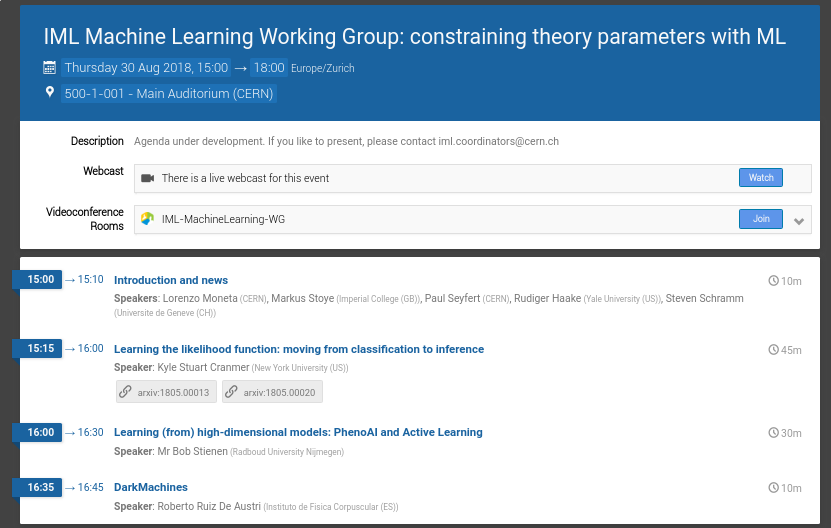
\includegraphics[width=.9\textwidth]{./agenda.png}
\end{frame}

\setbeamertemplate{background canvas}{%
  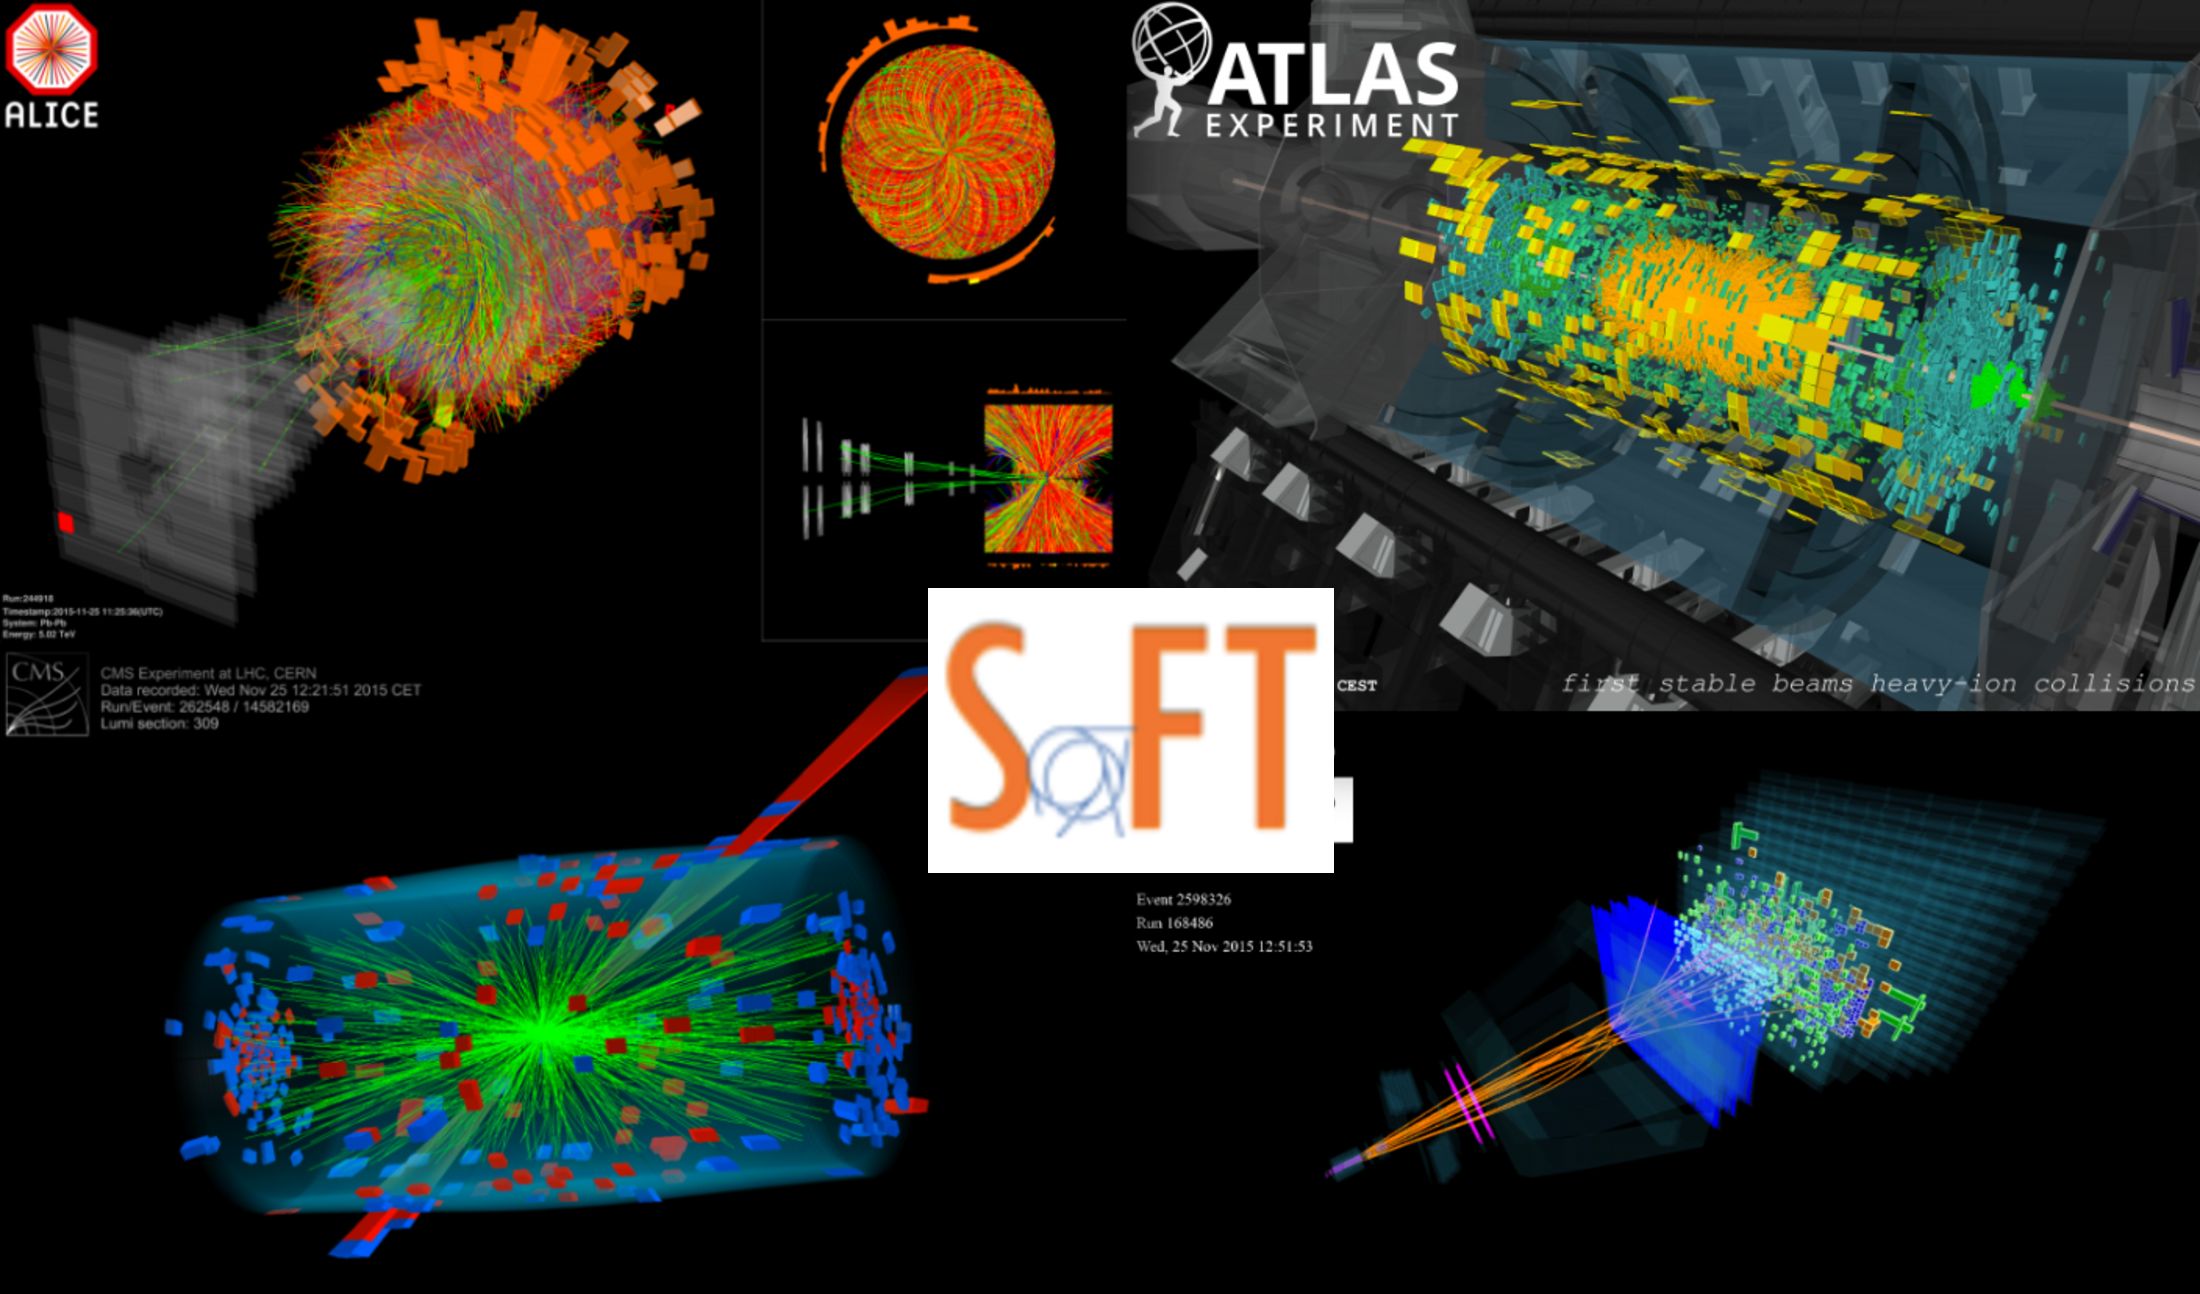
\includegraphics[width=\paperwidth,height=\paperheight]{banner.pdf}%
  }   
  \begin{frame}[t]
    \visible<2>{
      {~}
      \vspace{.5\textheight}
      \begin{columns}
        \begin{column}{.8\textwidth}
        \end{column}
        \begin{column}{.2\textwidth}
          \begin{block}{}
            \IfFileExists{./QR2.png}{
              \footnotesize{slides (excl.\ cern logo) will appear on}

              \gitlablink
\includegraphics[width=.2\textwidth]{./QR2.png}
            }{}
          \end{block}
        \end{column}
      \end{columns}
    }
  \end{frame}
  \beamertemplateshadingbackground{Black!03}{White}

  %
  % \appendix
  %
  % \begin{frame}
  %   \frametitle{BACKUP}
  %   backup is for people who can't improvise
  %
  %   (yes, that's a cheap excuse for not preparing backup slides)
  % \end{frame}
